\documentclass[11pt]{article}
\usepackage{amsmath}
\usepackage{anysize}
\usepackage[pdftex]{graphicx}
\marginsize{1in}{1in}{1in}{1in}
\begin{document}

\begin{flushright}
Zack Mayeda cs184-bg \\
Tyler Brabham cs184-ej
\end{flushright}

\begin{center}
\LARGE
Fluid Simulation Using Smoothed Particle Hydrodynamics
\end{center}

\section*{Abstract}
We explore the method of Smoothed Particle Hydrodynamics discussed by M. Kelager in [3] for the simulation of water and other interesting liquids, such as liquids with high viscosity and high surface tension. We use two different but related methods, Marching Cubes and Ray Marching, for surface reconstruction of the 
isosurface generated by the density field. For the former we utilize a library and for the latter we reuse a previously made ray tracer for Assignment 2 of CS184.  We found that although ray marching provides more interesting results, they come with a significant increase in computation time.

\section*{Introduction}
The idea behind SPH is that for each particle we can determine any desired scalar quantity by weighting that quantity from neighboring particles with an appropriate kernel function. The formula states that for any value of interest $A_i$ at particle $i$: $$A_i = \sum_{j} A_j \frac{m_j}{\rho_j}W({\bf r_{ij}},h)$$
where $m_j$ and $\rho_j$ are the mass and density of particle $j$, $W$ is a kernel function, $h$ is the support radius of $W$, and ${\bf r_{ij}}$ is the vector from particle $j$ to particle $i$. 
\\ \\
For example, to get the density of particle $i$, we substitute $\rho_j$ for the quantity of interest $A_j$. This tells us that: 
\\
$$\rho_i = \sum_{j} m_jW({\bf r_{ij}},h)$$

\section*{Solving Navier-Stokes Equation}
For each particle we need to update its position and velocity based on the current arrangement of particles. The equation we are solving to get the change in velocity of each particle is:
$$\rho_i \frac{dv_i}{dt} = - \bigtriangledown p_i + \mu \bigtriangledown^2 \cdot v_i + f_{external}$$
Thus, to get the values necessary to solve the Navier-Stokes equation, we need to know the density, pressure gradient, viscosity, and external forces acting on the particle, such as gravitational force and surface tension. Computing most of the desired quantities relies on knowing the density at each particle. Thus, we first loop through all particles and compute density, and then loop again to compute the remaining quantities.
\\
\\
The values we need in terms of our kernel method, in addition to the density calculation above, are then just:\\ \\
{\bf Pressure Gradient}
$$ - \bigtriangledown p_i = - \sum_{j}m_j \frac{p_i+p_j}{2\rho_j} \bigtriangledown W({\bf r_{ij}},h)$$
\\
where the $p_i$ and $p_j$ are pressures given by $p_i = k(\rho_i - \rho_0)$ with $\rho_0$ the ideal density of the fluid and $k$ a stiffness constant.
\\
\\
{\bf Viscosity}
$$ \mu \bigtriangledown^2 \cdot v_i = \mu  \sum_{j} m_j \frac{v_j-v_i}{\rho_j} \bigtriangledown^2 W({\bf r_{ij}},h) $$
\\
where $\mu$ is the viscosity coefficient of the fluid.
\\
\\
{\bf Surface Tension}
$$f_{tension} = -\sigma \bigtriangledown^2 c_i {\bf n_i}$$
\\
where $c_i$ is the color field calculated by plugging in $1$ for $A_j$ in the generic kernel form, and ${\bf n_i}$ is the normalized gradient of the color field.
\\
\\
{\bf Gravitational Force}
$$f_{gravity} = \rho_i {\bf g}$$
\\
We add up all these quantities in the Navier-Stokes equation and solve the equation for the change in velocity of particle $i$. Then we update the current velocity and position for each particle. To do this, we use Euler's method with a step size of $.01$.
We tried the method of Verlet as well, but experienced no change in the simulation, so we went back to using the simpler method. This perhaps would have not been the case had we used a larger timestep.

\section*{Kernels}
For our computations we use the following kernels as suggested from [1]. In all of the following, $h$ is the support radius of the kernel, ${\bf r_{ij}}$ is the vector from point $r_j$ to $r_i$, and $r$ is the length of this vector. For all the kernels, we use the below formulas provided $r\leq h$; otherwise, we return $0$.\\ \\
{\bf Default}
$$W({\bf r_{ij}},h) = \frac{315}{64\pi h^9}(h^2 - r^2)^3 $$ \\
The default kernel is used for all quantities except pressure and viscosity.
\\
\\
{\bf Pressure}
$$ W({\bf r_{ij}},h) = \frac{15}{\pi h^6}(h-r)^3$$
\\
We use this kernel only for calculating pressure gradient, so really we need the gradient of this kernel, which is:
\\
$$\bigtriangledown W({\bf r_{ij}},h) = \frac{-45}{\pi h^6}\frac{{\bf r_{ij}}}{r}(h-r)^2$$
\\
We use this kernel for pressure because the magnitude of $\bigtriangledown W$ is nonzero as $r$ approaches $0$.
\\
\\
{\bf Viscosity}
$$W({\bf r_{ij}},h) = \frac{15}{2\pi h^3}(-\frac{r^3}{2h^3} + \frac{r^2}{h^2} + \frac{h}{2r} - 1) $$
\\
Similar to pressure, we really need the laplacian of this kernel for the viscosity calculations. The laplacian is:
\\
$$\bigtriangledown^2 W({\bf r_{ij}},h) = \frac{45}{\pi h^6}(h-r) $$


\section*{Improving Computation Time}
A  na\"{\i}ve implementation of a fluid simulation using SPH takes into account interaction between all pairs of particles each time step, producing a runtime of $O(n^2)$, where n is the number of particles. To speed up the simulation, we used the nearest neighbor algorithm which assumes that particles will only interact if they are within a certain distance of each other, the radius of support. This radius, which is the same as the support radius of the kernels, can be adjusted so that the fluid simulation produced looks identical to the simulation produced by the  na\"{\i}ve implementation. Using this algorithm, the runtime is reduced to an expected runtime of $O(nm)$, where m is the average number of neighbors of each particle.

\section*{Explicit Constants}
In the following table we list all the constants we used for simulating water. To simulate other more viscous fluids we just vary the values in the table below to preference. In addition to those listed, we use a length tolerance of $6.0$ for the surface tension calculation; ie, if the length of the surface normal is less than the tolerance we do not include it in the calculation.

\begin{center}
    \begin{tabular}{| l | l | l | l |}
    \hline
    Mass & .02 \\ \hline
    Stiffness & 3.5\\ \hline
    Ideal Density & 1000 \\ \hline
    Viscosity & 3.5\\ \hline
    Surface Tension & .07 \\ \hline
    Support Radius & .0625 \\ \hline
    \end{tabular}
\end{center}
The majority of these constants come from [3], which also has recommended constants for other fluids, such as mucous. One could consult those constants if interested in replicating those results.


\section*{Surface Reconstruction}
To reconstruct the surface we use an isosurface level of 500. Although 1000 would be more physically accurate for water, we found the results for 1000 to make the water appear significantly more globular and compressible, and less like actual water. For this reason it would seem the method of SPH is more suited for compressible fluids.
\\
\\
For the first method of surface reconstruction with Marching Cubes, we used a standard implementation from [2]. The algorithm breaks up the container of the fluid into a grid and considers the density value at each of the eight vertices of a cube in the grid. Depending on which vertex densities are above a certain threshold we have different cases to consider for how to draw the triangles. We implemented the marching squares version ourselves for 2D simulation (which requires considering 16 different cases when drawing triangles) but relied on the implementation from [2] to perform marching cubes (which requires 256 cases).
\\
\\
For the second method, we reused a ray tracer written for a previous assignment. We extended our Shape superclass (the parent class of our Ellipsoid and Triangle classes) to a subclass called ParticleBlob and implemented a new intersection checking method using ray marching. To determine the density and normal vector at a point we reuse the kernel functions from the SPH simulation. In addition, we reuse the neighbor structure to accelerate the processing of the particles within the ray tracer. With this ray tracer we were able to generate much more interesting images, which used reflections and refractions. But the computation cost of using ray marching for the surface reconstruction was significantly higher than that of Marching Cubes.


\section*{Results}
Resulting images can be seen in the figures at the end of the document.  A video is temporarily available at http://inst.cs.berkeley.edu/$\sim$cs184-bg/.
\\ \\
The simulation using only particles rendered as spheres took approximately .287 seconds per frame on the scale of 2k particles, and 55 seconds per frame on the scale of 100k particles, depending on the distribution of the particles in the container. Two images created with the higher particle count are shown in figure 1. The video contains both low and high particle count for comparison. 
\\ \\
When reconstructing the surface with marching cubes, it took around 22, 600, and 2100 seconds per frame when rendering 2k, 21k, and 45k particles, respectively. Images created on the 2k and 21k scale can be seen in figure 5. Note in the figure that the surface appears very globular. As such, it would seem SPH is not as well suited for the simulation of lower viscosity fluids. Also, due to the nature of the density grid, the fluid appears to be very compressible. As particles approach the side of a container, the fluid surface near the container disappears as opposed to being deformed. This is more easily seen in the video.
\\ \\
As for ray marching, the reconstruction of the surface is very slow, even on the scale of 600 by 600 pixels. With around 2k particles, the average time per frame is 440 seconds, compared to the 22 seconds for marching cubes. Figures 2, 3, and 4 show ray traced images in similar scenes. Particularly in figure 4 the reflection and refraction of the container are very noticeable.

\section*{Conclusion \& Future Consideration}
In this project, we implemented the Smoothed Particle Hydrodynamics method of fluid simulation, in particular for the simulation of liquids. We explored a couple different methods for surface reconstruction, and found neither to be sufficient for the simulation of incompressible fluids. In addition, the surface reconstruction significantly added computational cost to the simulation, preventing it from rendering at a reasonable frame rate, even with the acceleration obtained from implementing the Nearest Neighbors algorithm for the particle interactions.
\\ \\
The project was a fun first foray into fluid simulation. In the future, we would like to try other methods such as an Eulerian method, and improve the speed of the current program by including parallel processing of the particles. As well, including reflection and refraction of the surface is only part of the reproduction of water, so we would like to include realistic caustics in future projects.

\begin{figure}
\begin{center}$
\begin{array}{c}
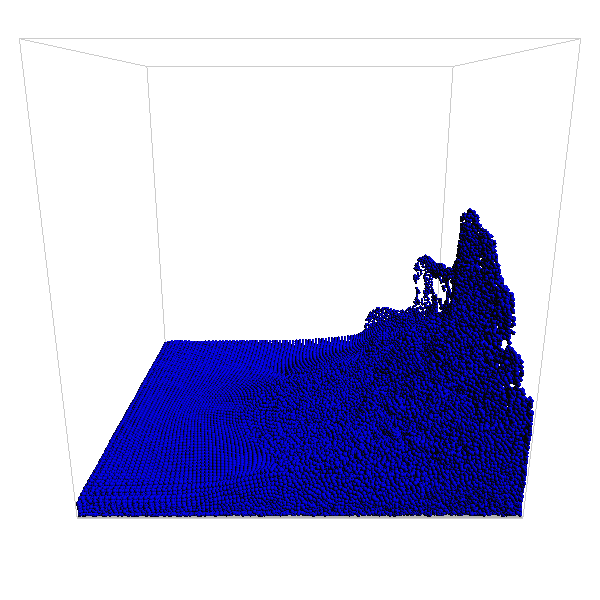
\includegraphics[width=4in,height=4in]{97k-particles.png} \\
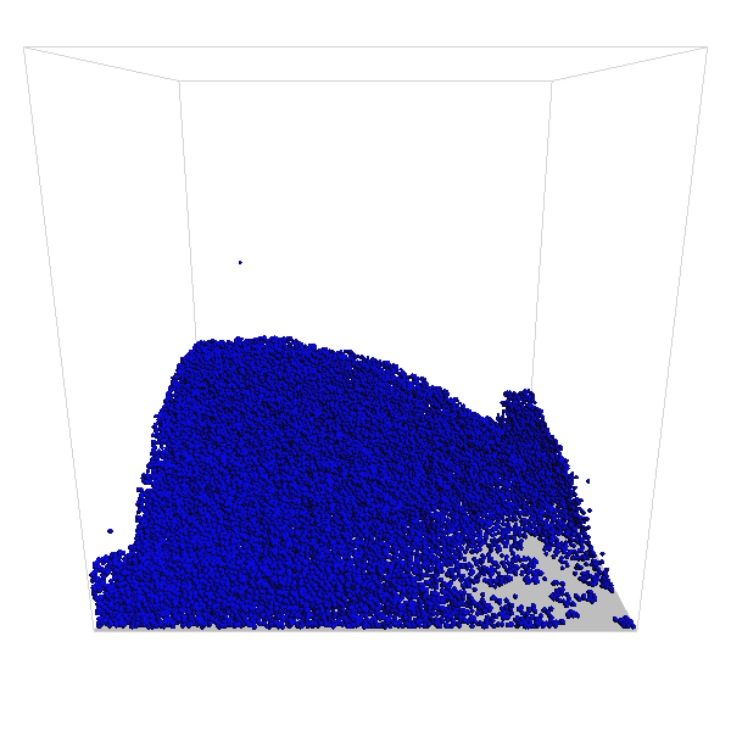
\includegraphics[width=4in,height=4in]{79k-particles.pdf}
\end{array}$
\end{center}
\caption{The first image shows 100k particles initialized with a rightward velocity, and the second image shows 80k particles released from a stationary cube at the back left corner of the container.}
\end{figure}

\begin{figure}
\begin{center}$
\begin{array}{cc}
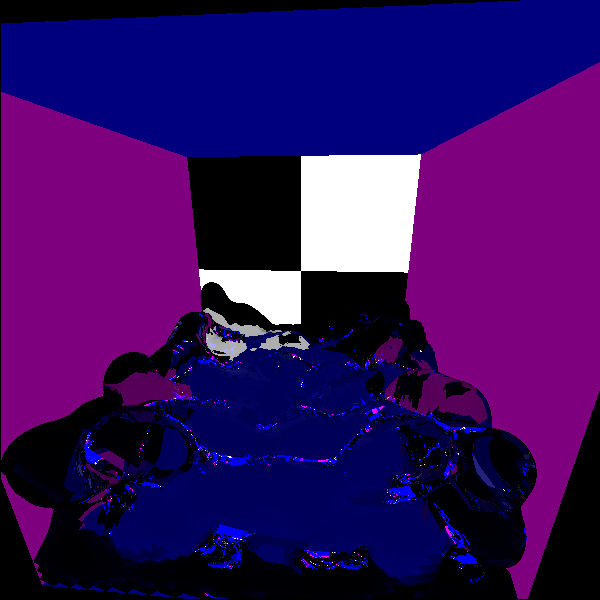
\includegraphics[width=3in,height=3in]{2k-ray-active.png} &
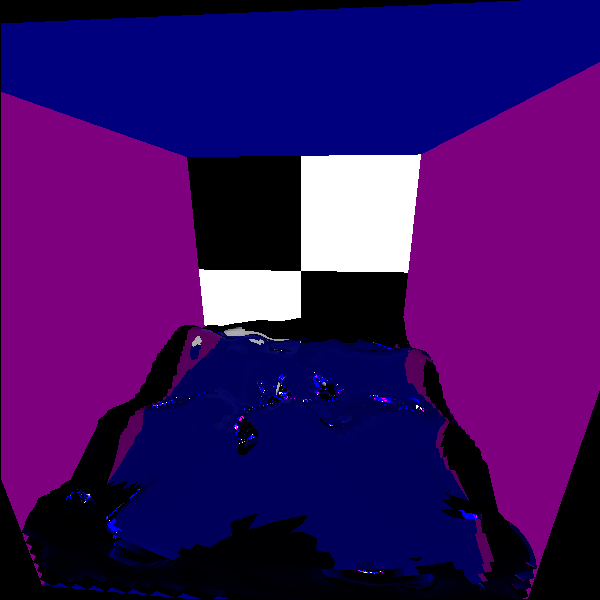
\includegraphics[width=3in,height=3in]{2k-ray-settled.png}
\end{array}$
\end{center}
\caption{Two ray traced images a few frames apart in the scene. The image shows refraction and reflection.}
\end{figure}

\begin{figure}
\begin{center}$
\begin{array}{c}
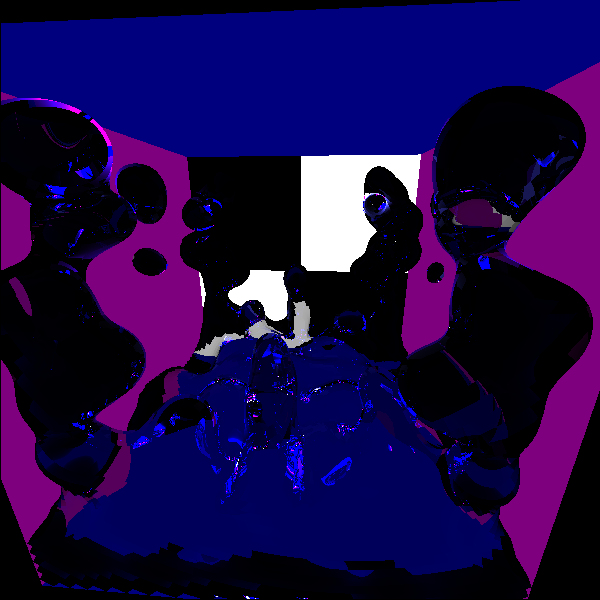
\includegraphics[width=4.4in,height=4.4in]{towers.png}
\end{array}$
\end{center}
\caption{Another look at a ray traced image.}
\end{figure}

\begin{figure}
\begin{center}$
\begin{array}{c}
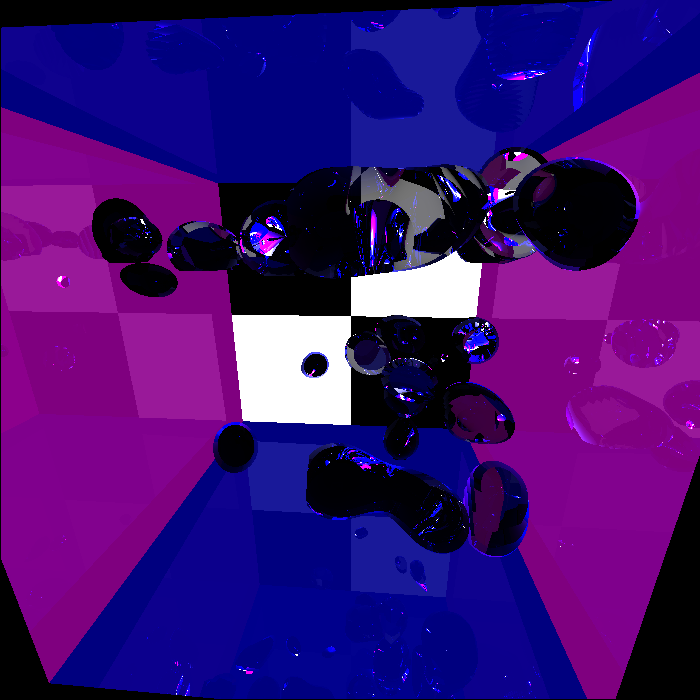
\includegraphics[width=6in,height=6in]{raytrace.png}
\end{array}$
\end{center}
\caption{Another ray traced image with more noticeable refraction and higher level of reflections.}
\end{figure}

\begin{figure}
\begin{center}$
\begin{array}{c}
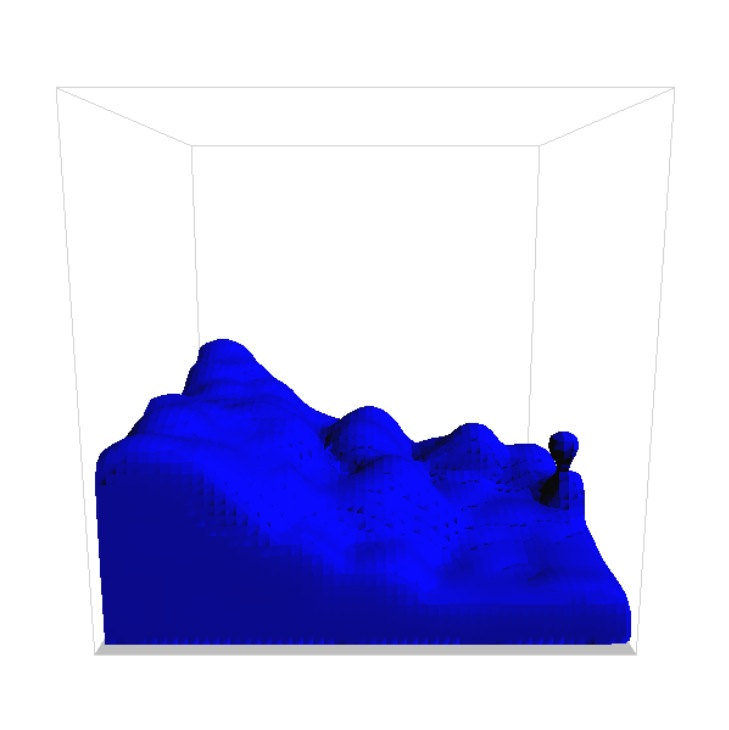
\includegraphics[width=4in,height=4in]{18ke-1-march.jpg} \\
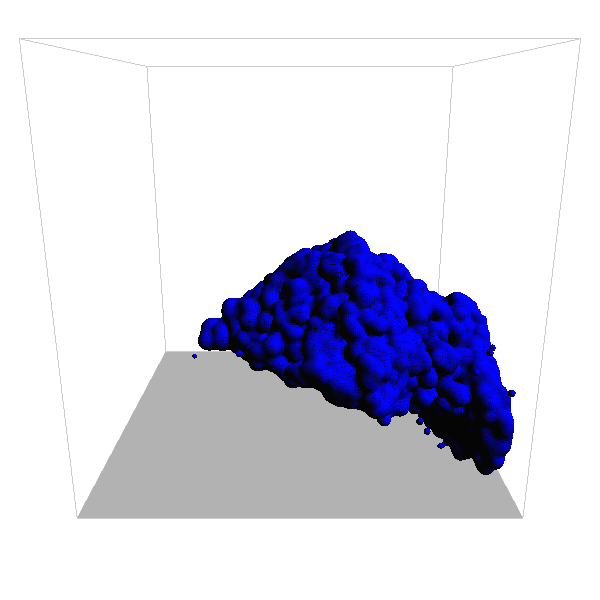
\includegraphics[width=4in,height=4in]{21k-march.png}
\end{array}$
\end{center}
\caption{The image on the top uses 1.8k particles, while the image on the bottom uses 21k. Note the reconstructed surface appears globular, particularly for the image on the bottom.}
\end{figure}

\begin{thebibliography}{5} 
\bibitem{PRESENT} Auer, S., ``Realtime Particle-Based Fluid Simulation", Computer Graphics and Visualization, October 4th, 2008.
\bibitem{Matt} Fisher, M., Stanford: Matt's Webcorner, 
\\ http://graphics.stanford.edu/$\sim$mdfisher/MarchingCubes.html, accessed April 20th, 2013.
\bibitem{Kelager} Kelager, M., ``Lagrangian Fluid Dynamics Using Smoothed Particle Hydrodynamics," \emph{Department of Computer Science, University of Copenhagen}, January 9th, 2006.
\end{thebibliography}

\end{document}{l c r}